\documentclass[10pt]{proc}

\usepackage{amsmath}    % need for subequations
\usepackage{graphicx}   % need for figures
\usepackage{verbatim}   % useful for program listings
\usepackage{color}      % use if color is used in text
\usepackage{subfigure}  % use for side-by-side figures
\usepackage{hyperref}   % use for hypertext links, including those to external documents and URLs
\usepackage{multicol}

\author{P.~Gusev, J.~Burke}
\title{NDN-RTC Technical Report (draft version)}

\begin{document}

\maketitle

%************************************************
\abstract
TBD

%************************************************
\section{Introduction}
TBD

%************************************************
\section{Background and prior work}
TBD

%************************************************
\section{Goals}
TBD

%************************************************
\section{Architecture}
There are two parties involved in RTC communication over NDN: producer and consumer. In presence of NDN network the paradigm of RTC shifts from the push-based (when producer writes data to the socket and consumer reads it as fast as possible) to the pull-based (producer publishes data on the network with his own pace, while consumer has to request the data he needs and manage incoming data segments).
Producer's main task is to grab media data from media inputs, encode it, pack into network packets and store it in the cache for predefined data freshness period, after which data is removed from the cache.
Consumer implements more sophisticated algorithms for achieving following goals:
\begin{itemize}
\item ensure fetching the latest data from the network; 
\item playback fetched media in correct order;
\item handle network latency and packet drops.
\end{itemize}

\begin{figure}[Ht!]
\centering
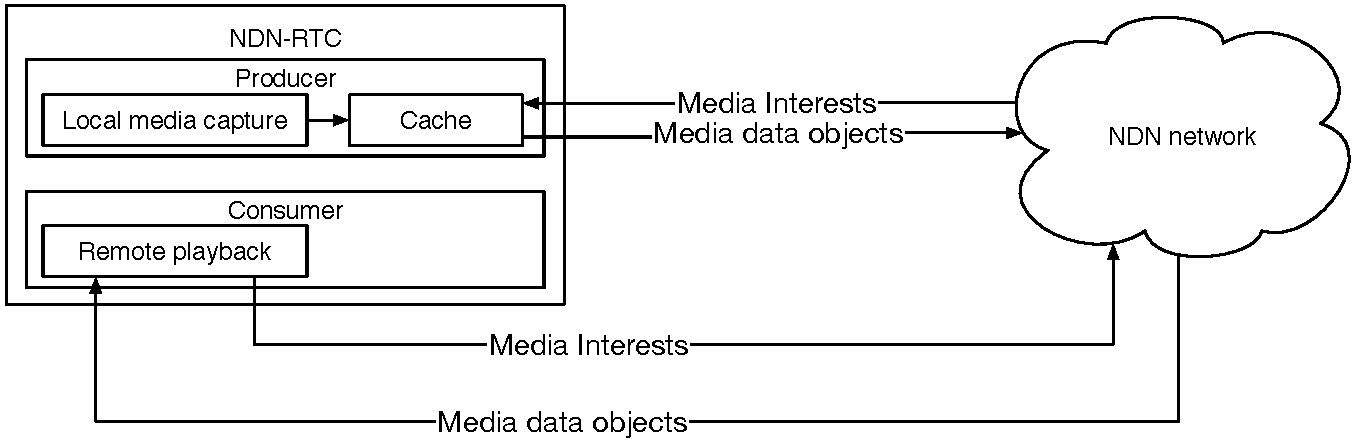
\includegraphics[width=0.5\textwidth]{architecture}
\caption{RTC over NDN}
\label{fig:arc}
\end{figure}

Figure \ref{fig:arc} presents top-level overview on how NDN-RTC works. Local media capture and Cache belong to the producer part of the NDN-RTC. Media is stored in the cache which provides access to the data for all incoming interests. Remote playback represents consumer: it issues interests, prepares received media and plays it back.

\paragraph{Producer}

In case of video streaming, individual encoded frames can vary in size. For example, 1000 kbps stream produces two types of frames:
\begin{itemize}
\item \textbf{Key frames} - about 30KB in size;
\item \textbf{Delta frames} - from 1 to 7KB in size. 
\end{itemize}

As current NDN implementation works on top of the IP network, data chunks can not exceed standart MTU size of 1500 bytes. Therefore producer, as seen on Figure \ref{fig:producer}, should segment encoded frames into smaller data chunks.

\begin{figure}[Ht!]
\centering
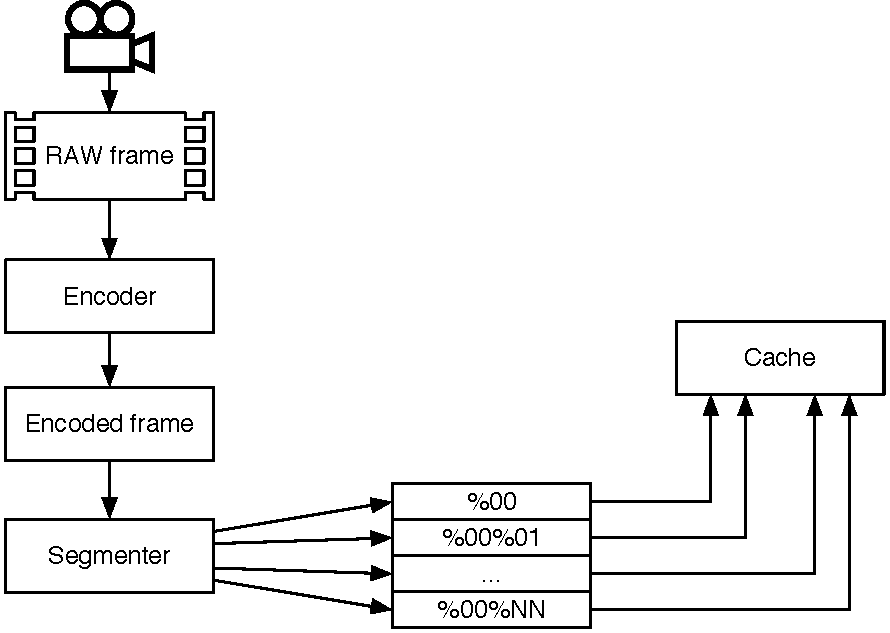
\includegraphics[width=0.5\textwidth]{producer}
\caption{NDN-RTC producer}
\label{fig:producer}
\end{figure}

\paragraph{Consumer}

Consumer takes into account that media packets are presented by separate segments in the network. Therefore, consumer implements mechanisms of interest pipeliner and frame buffer (see Figure \ref{fig:consumer}). Interest pipeliner issues interests for individual segments and is controlled by some higher-level logic for ensuring that only the latest data is fetched, thereby first out of three consumer's goals is achieved. Other two goals are attained by frame buffer which handles network latency by introducing some buffering delay and out-of-order packets arrival by organizing received frames in the proper order. 

\begin{figure}[Ht!]
\centering
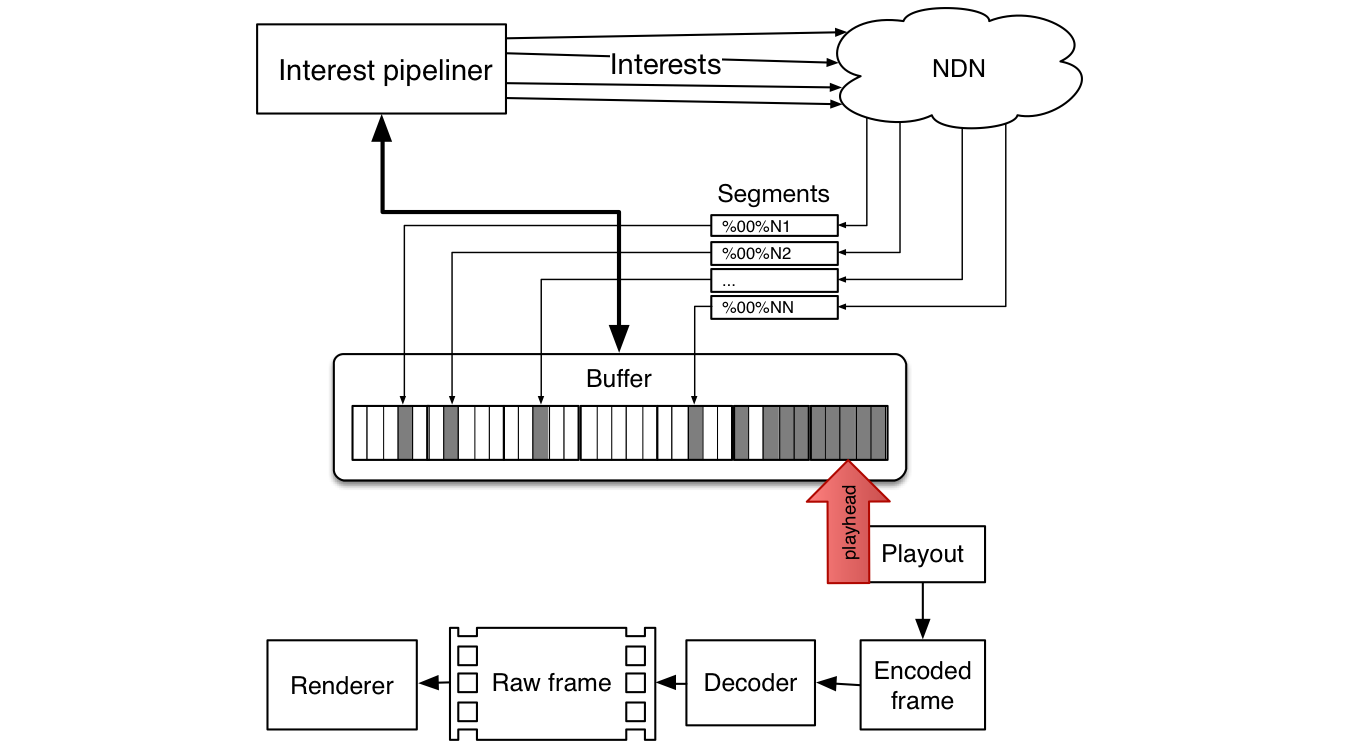
\includegraphics[width=0.5\textwidth]{consumer}
\caption{NDN-RTC consumer}
\label{fig:consumer}
\end{figure}


%************************************************
\subsection{Namespace}

Each user of NDN-RTC app is uniquely identified by a prefix URI which contains username (producer id on root level on the Figure \ref{fig:namespace}). A user publishes her media streams (audio or video) under streams namespace as presented in Figure \ref{fig:namespace}. Producer can publish one particular stream in several copies with different encoding parameters (for instance, to allow consumers fetch media stream wich is the most appropriate for current network conditions). The information about streams’ encoding parameters can be accessed by issuing interest in producer's \texttt{codec\_info} namespace (\textbf{/$<$user prefix$>$/streams/video0/vp8/codec\_info}).
Any user who wants to fetch producer's media stream needs to express interest with URI corresponding to a certain media stream.

\begin{figure}[Ht!]
\centering
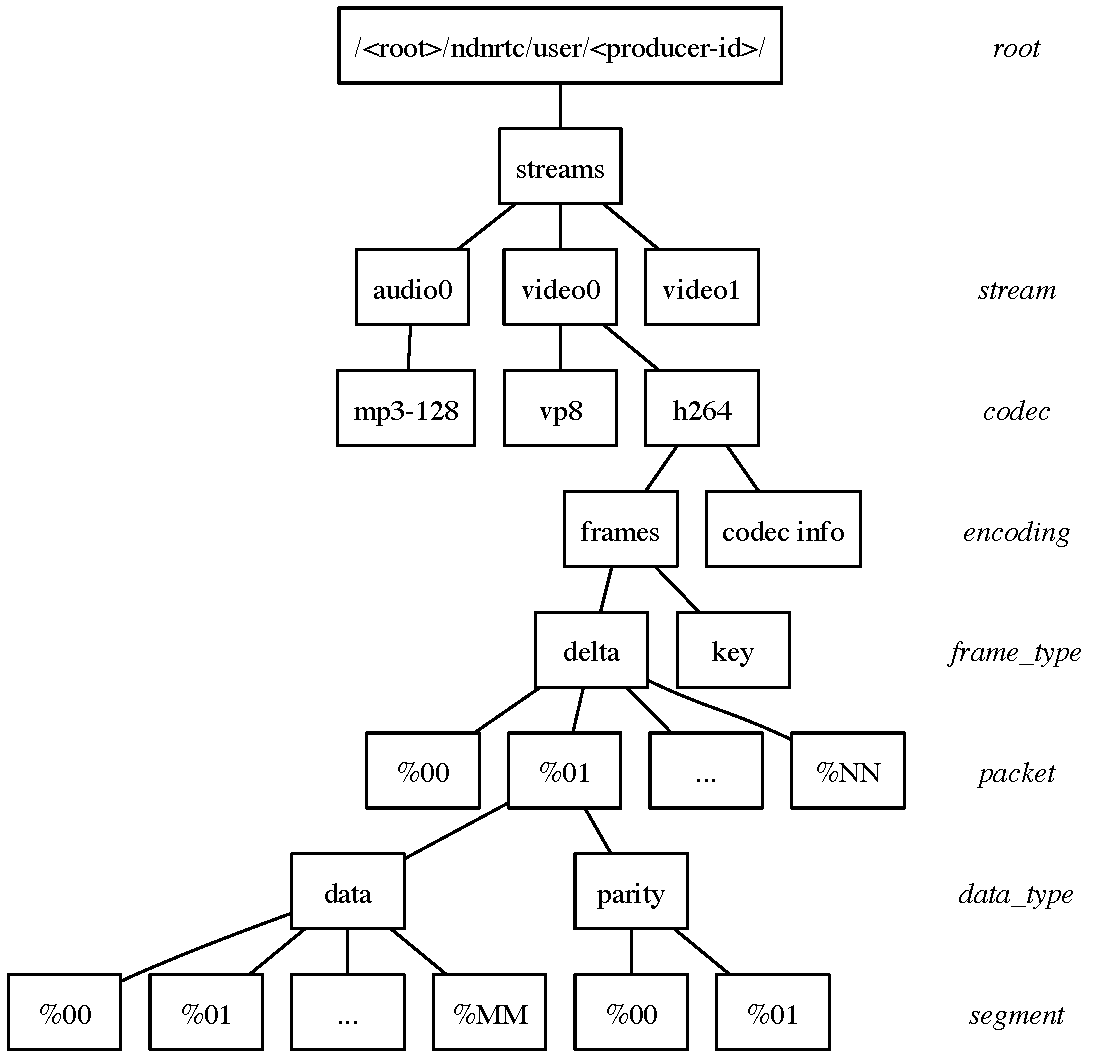
\includegraphics[width=0.5\textwidth]{namespace}
\caption{NDN-RTC namespace}
\label{fig:namespace}
\end{figure}

%************************************************
\subsection{Consumer protocol}

%************************************************
\subsubsection{Frame fetching}

In order to understand principles underlying consumer protocol, let's analyze frame fetching process (see Figure \ref{fig:pull}). As was noted before, frames are made of several segments. This number of segments is not known beforehand, unless the very first segment is fetched - in this case, consumer can retrieve metadata from the received packet (see Table \ref{tab:meta}) and get total number of segments for current frame. Therefore, at first attempt, consumer tries to "guess" the number of segments she needs to fetch by issuing $M$ interests (see Figure \ref{fig:pull}). These interests can arrive to producer before request frame is published and stay in the cache for some amount of time $d_{gen}$ called \texttt{generation delay}. Once the frame is segmented into $N$ segments and these segments are published, interest $0 - M$ are answered with the data which travels back to consumer. Upon receiving first data segment, consumer retrieves metadata from received segment and determines total number of segments for current frame. In case if $N > M$, consumer issues more $N - M$ interests for missing segments. These segments will be satisfied with data with no generation delay. The time interval between receiving very first segment and until frame is fully assembled is represented by $d_{asm}$ and called \texttt{assembling time}.

\begin{figure}[Ht!]
\centering
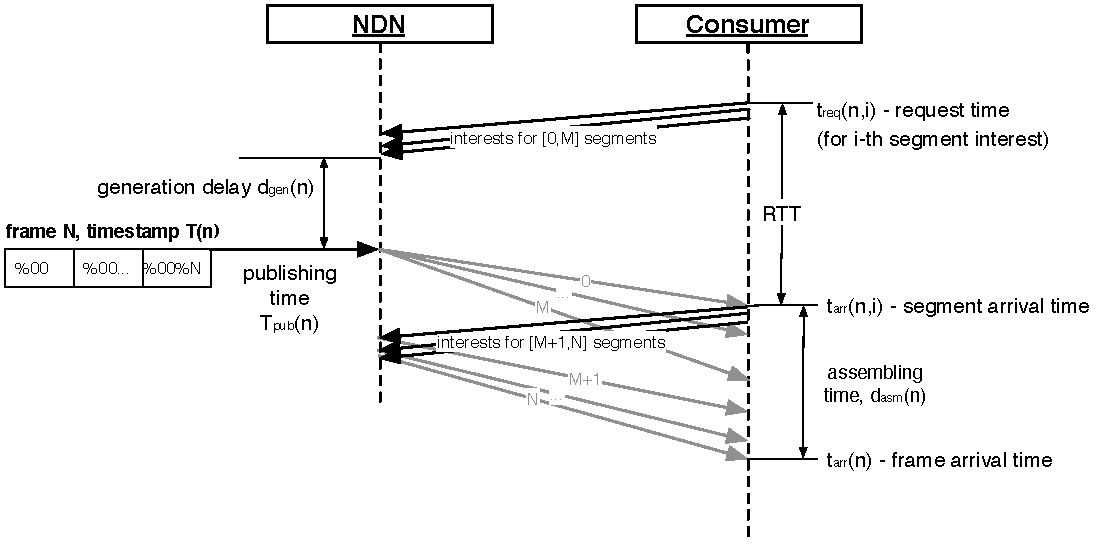
\includegraphics[width=0.5\textwidth]{frame-fetch}
\caption{Fetching frame}
\label{fig:pull}
\end{figure}


Clearly enough, consumer is interested in minimization of assembling time. First version of library was designed to have fixed amount of initial interests for all frame types. This caused problems, depicted on Figure \ref{fig:fetch-key}. Key frames are much larger than delta frames and this implies longer assembling times for key frames. However, consumer doesn't know what kind of frame she fetches next and experiments showed that quite often key frames did not have time enough to be assembled by the time they should be played back. This problem was solved by adding following considerations:
\begin{itemize}
\item consumer should know what type of frame she is going to fetch;
\item consumer should track average number of segments per frame type.
\end{itemize}

The first consideration was implemented by introducing separate namespaces for key and delta frames. The second consideration helps consumer make a "best guess" on number of initial interests to be issued in order to keep assembling time minimal.

\begin{figure}[Ht!]
\centering
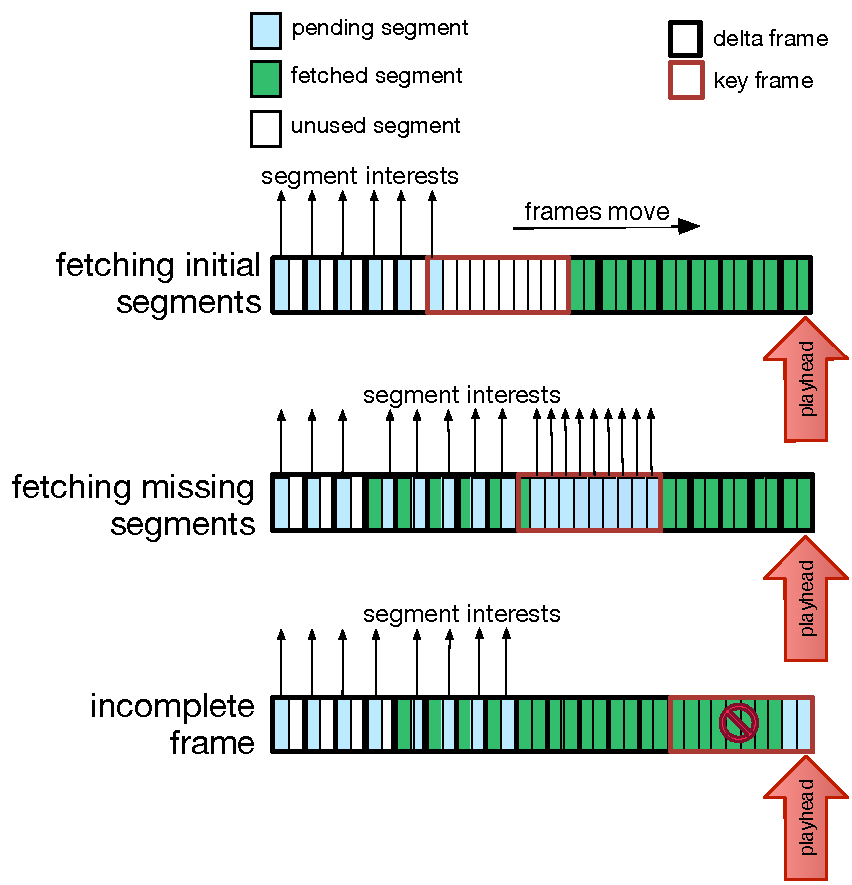
\includegraphics[width=0.5\textwidth]{key-fetch}
\caption{Fetching key frame}
\label{fig:fetch-key}
\end{figure}


\subsubsection{Bufferization}

Pull-based one-to-many media data fetching results in different bufferization mechanisms for the consumer. Consumer should be aware that the data requested could not come earlier than the RTT value for the current network topology (see Figure \ref{fig:pull}), assuming that data has been already placed in the content store of forwarder by the time it received the interest. Moreover, RTT values can vary greatly (order of magnitude) depending on how far in the network interest should go (in case there are several hubs between consumer and producer). Clearly, consumer should be aware of this fact and take this into consideration while performing measurements. However for now, we assume that RTT values will not vary greatly.

Consumer is interested in getting the most recent data from the network. Taking into account RTT value, consumer should express interests in such a way, that they could arrive to the producer as close as possible to the frame publishing time $T^{pub}_{n}$. In general, RTT value for the $i$-th interest of the $N$-th frame can be expressed by the following equation:
\begin{equation}
RTT_{ni} = t^{arr}_{ni} - t^{req}_{ni}
\end{equation}
where $t^{req}_{ni}$ - timestamp when the interest for $i$-th segment of $N$-th frame was expressed, $t^{arr}_{ni}$ - timestamp when the $i$-th data segment of $N$-th frame was received.

From the other point of view, RTT value can be represented like this:
\begin{equation}
RTT_{ni} = \widehat{RTT} + d^{gen}_{ni} + w_i
\end{equation}
where $\widehat{RTT}$ - real RTT value for the current network conditions, $d^{gen}_{ni}$ - delay between the moments when the interest has reached producer and requested data has been added to the content store, $w_i$ - network-introduced delay.
Whereas $w_i$ component cannot be omited entirely (though can be tracked), $d^{gen}$ is the variable that should be minimized by consumer in order to get the most accurate RTT estimation for the current network. 

Knowing RTT value is important for the consumer due to several reasons:

\begin{itemize}
\item consumer can estimate which fame number to request in order to get the latest data;
\item consumer can track segments arrival and set a deadline when a frame should be assembled and re-express interests for missing segments so that they can still arrive in time in order to finalize the frame.
\end{itemize} 

As network does not guarantee packet delivery, consumer should be aware of data losses and incorporate this knowledge in bufferization mechanisms. 

Proposed frame buffer is presented on Figure \ref{fig:buffer}. This is a circular buffer with frames being assembled while moving from the left side (beginning) to the right side (end) of the buffer. New frames (recently requested by issuing interests) enter buffer in the beginning of the buffer and exit in the end of the buffer. Further, we will analyse and measure different frame positions inside the buffer using time scale (milliseconds), i.e. if the buffer size is $B$ milliseconds, then the frame $F_n$ which should be played back at the time $t_n$ has entered the buffer at the time $t_n-B$.

In order to understand, how buffer size should be determined, let's apply reasoning, explained in next paragraph.

To handle data losses, buffer needs a retransmission check point at which interests for the missing frame segments can be re-expressed. This checkpoint should be placed far enough from the point when the frame should be played back so the missing data could arrive by this time. Any expressed interest is expected to bring data segment in $\overline{RTT}$ milliseconds (where $\overline{RTT}$ - consumer's estimation of the current RTT value). Therefore, retransmission checkpoint should be placed at least $\overline{RTT}$ milliseconds earlier before the end of the buffer (playback deadline). The same reasoning could be applied to determine a point in time at which initial interests should be expressed (i.e. beginning of the buffer). In ideal network conditions (with no losses), re-transmission of interests for missing segments should not be required, i.e.  frame should have been already assembled by the time of retransmission checkpoint. This means that the point of time for initial interests issuing should be placed $\overline{RTT}+\overline{d^{asm}}$ milliseconds earlier than retransmission checkpoint, where $\overline{d^{asm}}$ - is the observed average assembling time for this specific frame type (as it can vary greatly depending on frame type - Key or Delta). Therefore, according to the Figure \ref{fig:buffer}, the values of $P$ (pipeline size of the buffer) and $J$ (jitter size of the buffer) should satisfy these inequalities:

\begin{equation}
P \geq \overline{RTT} + \overline{d^{asm}}; J \geq \overline{RTT}
\end{equation}


\begin{figure}[Ht!]
\centering
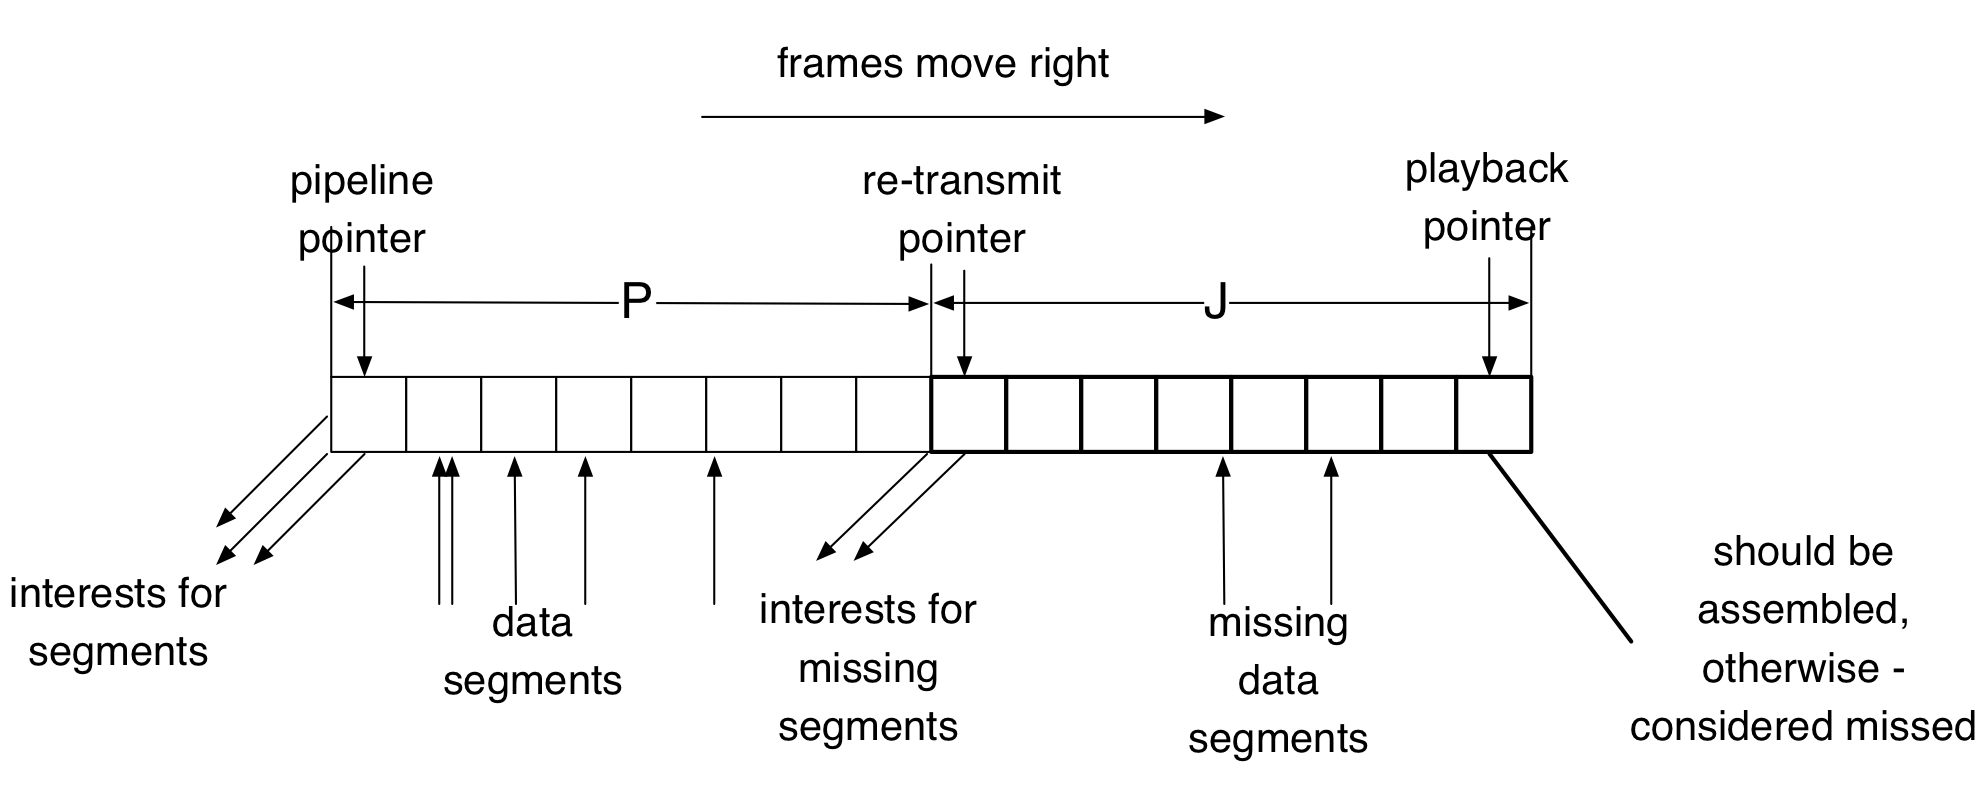
\includegraphics[width=0.5\textwidth]{buffer}
\caption{Frame buffer}
\label{fig:buffer}
\end{figure} 

\subsubsection{Interest pipeline}
One of the main goals for the consumer - express interests in proper time so that they can reach content store right before the requested data will become available. 
Consider Figure \ref{fig:int-expression}: interests for the frame segments are issued with interval $d^{int}$, assembled frames arrive to the buffer with the interval $d^{arr}$. Consumer can adjust $d^{int}$ value in order to get recent data. By tracking values of $\overline{RTT^{F}_i}$ for the $i$-the frame and arrival delay $d^{arr}$, consumer can infer adjustments needed for $d^{int}$. 
TBD

%\begin{figure}[Ht!]
%\centering
%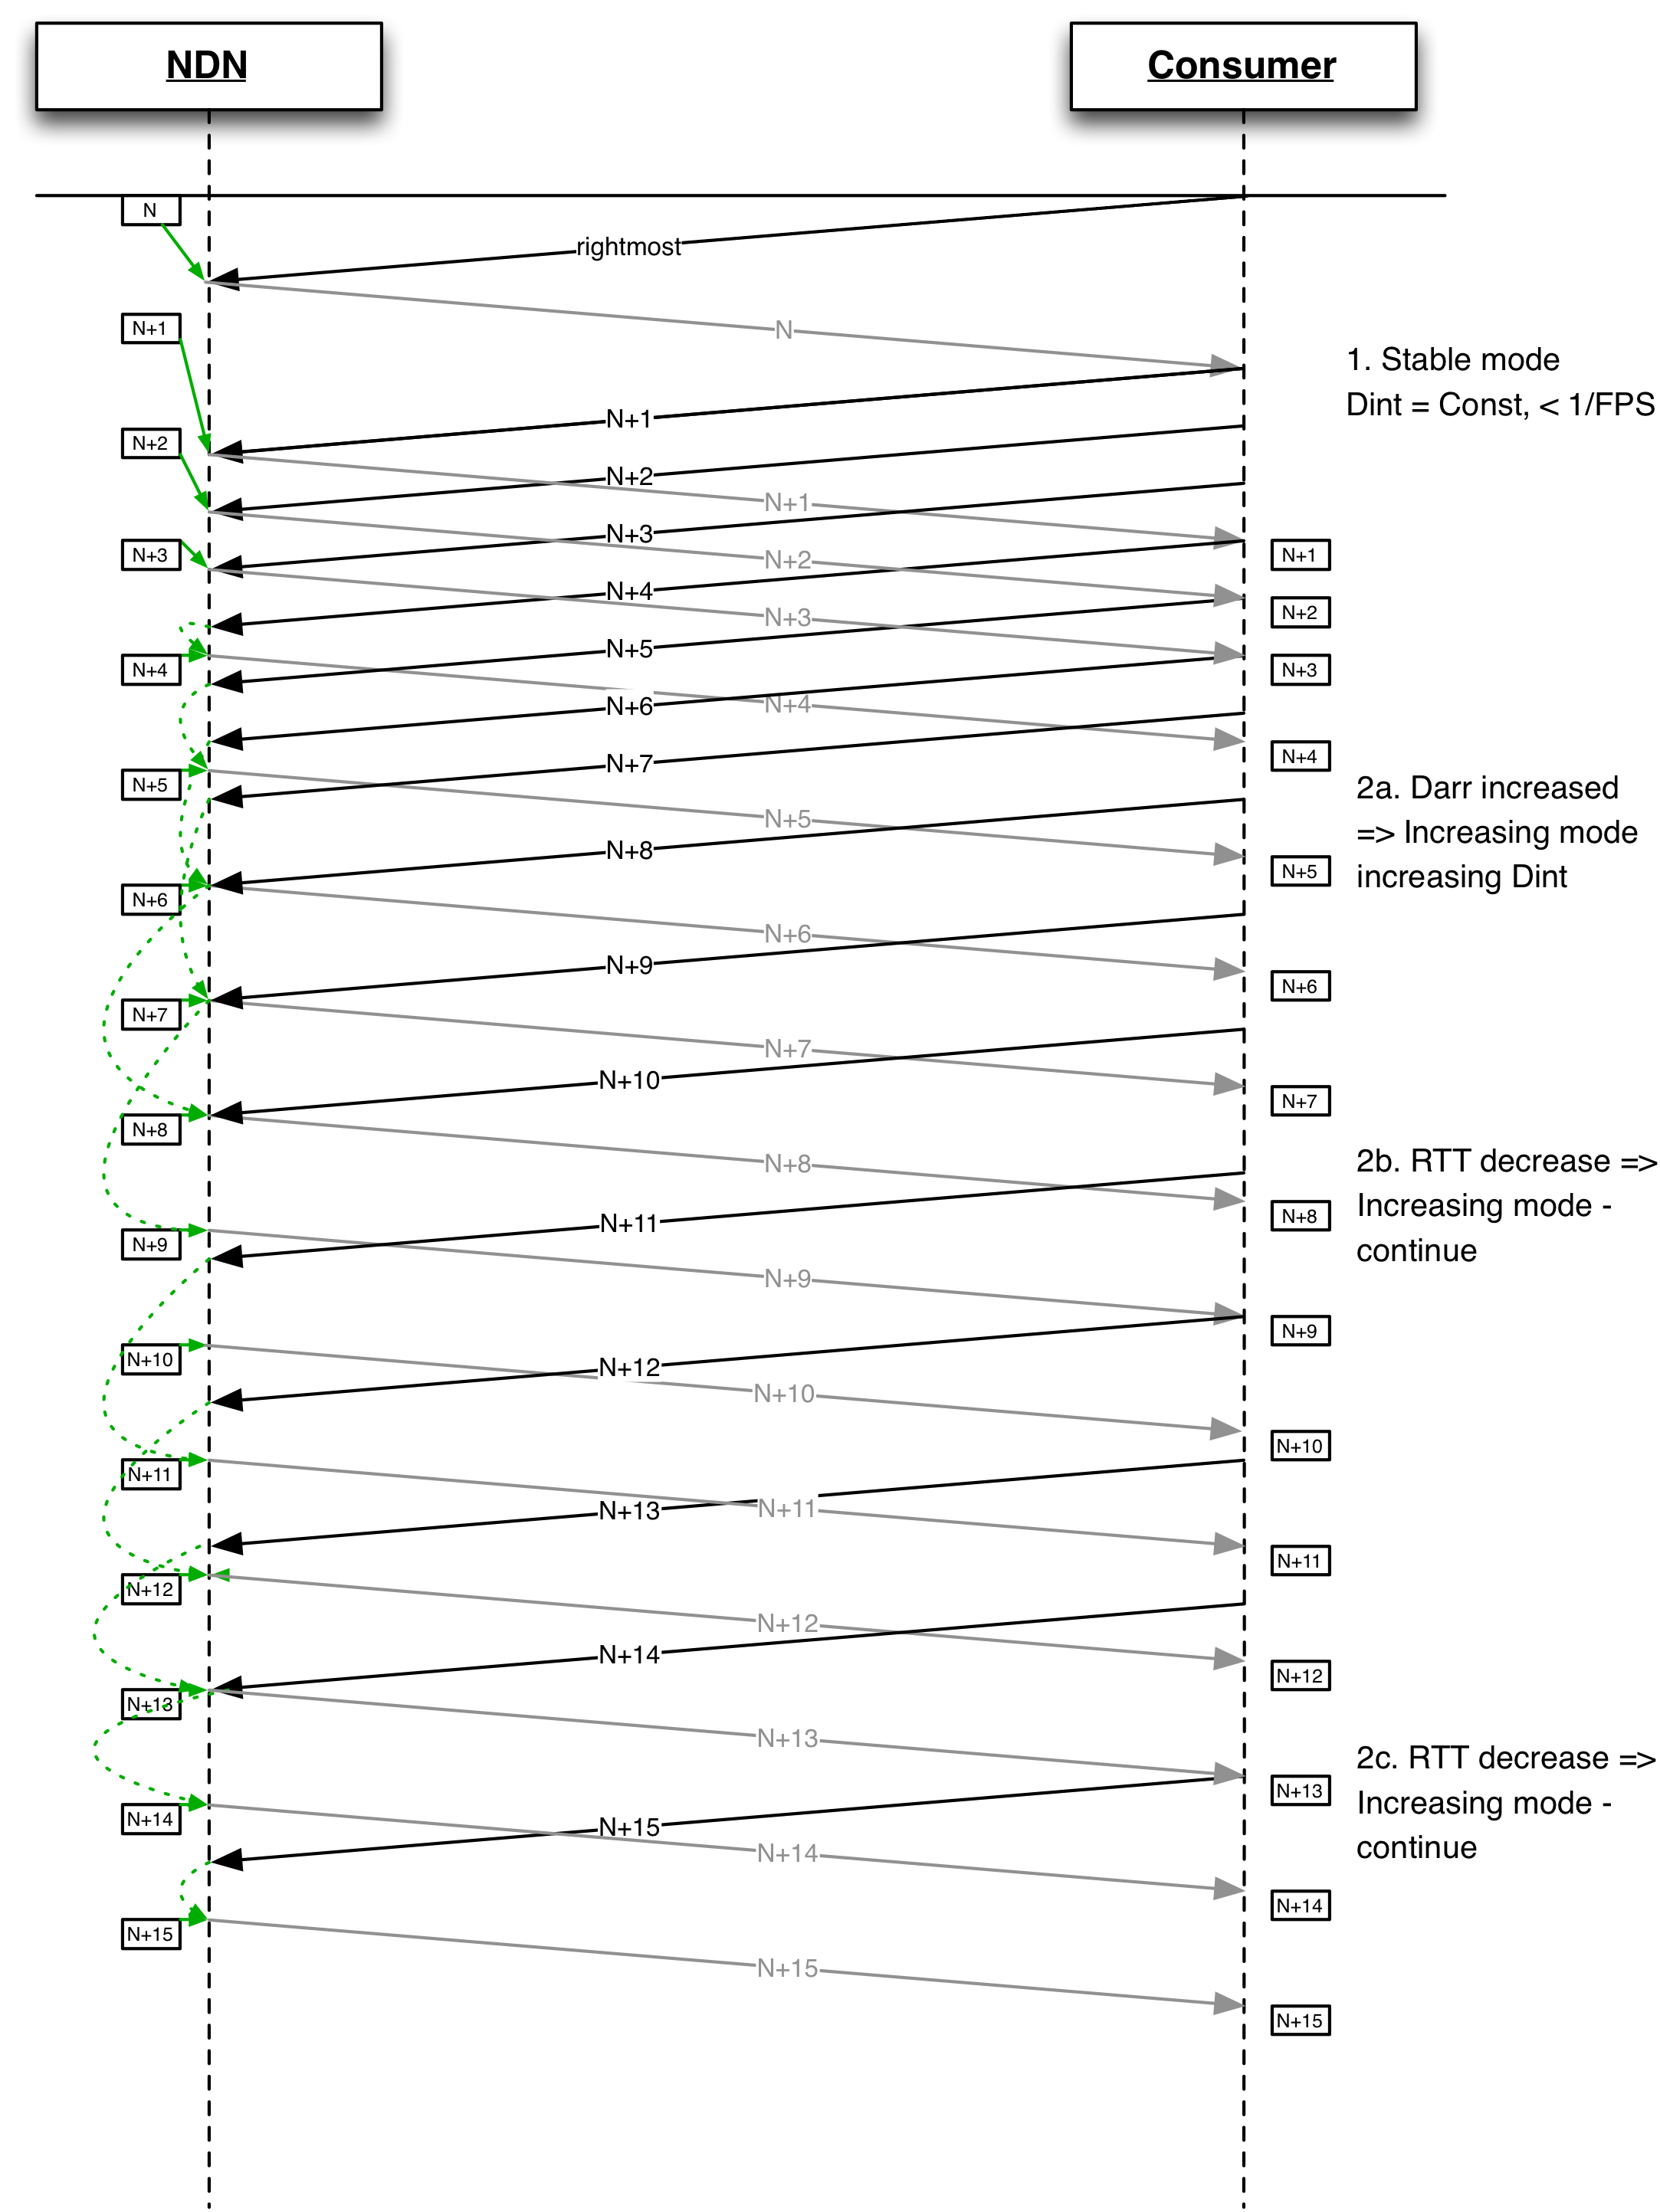
\includegraphics[width=0.5\textwidth]{pipeliner}
%\caption{Pipelining mechanism (TBD)}
%\label{fig:pipeliner}
%\end{figure} 

\subsubsection{RTT estimation}
TBD

\section{Implementation}
TBD

\section{Evaluation}
TBD

\section{Issues and future work}
TBD

\section{Conclusion}

\end{document}